\section{Детекторы}

\subsection{Электромагнитный калориметр}

Оригинальная идея считывать свет из слоистого калориметра посредством
спектросмещающих волокон (WLS) предложена в 1985 году Фесслером \cite{Fessler-Shashlik-1985}.

Идея была впервые реализована в виде гетерогенного ячеистого калориметра в
1991-1992 годах в ИЯИ РАН для эксперимента E-865~(BNL, США) \cite{BADIER199474}.
% ^^^ проверить, впервые ли -- доклад Гущина (см. слайд №5) выглядит
% пристрастным: http://www.inr.troitsk.ru/rus/kud-sem/gushchin26-03-12.pdf
% Встречал упоминание о гетерогенном калориметре CDF (Fermilab), 1988, где
% при толщине 18 X_0 Pb/scint разрешение составляло 13.5%/\sqrt{E}
% KLOE использовали 15 X_0 с файберами в 1995 5.7%/\sqrt{E} + .6%
В последующие годы калориметры такого типа получили широкое распространение за
счёт ряда технологических преимуществ~\cite{grupenDetectors2008}.
К числу таких преимуществ относятся:

возможность создания калориметра под необходимый мольеровский радиус,
позволяющий производить пространственное
разделение ливней от различных частиц, высокая радиационная
стойкость, устойчивость отклика при работе в магнитном поле,
стабильное энергетическое разрешение и высокая скорость отклика во
многих случаях позволявшая включать такой калориметр в триггерную систему.
Идея нашла применение во многих экспериментах:
PHENIX (BNL), LHCb, DELPHI, CMS, COMPASS (CERN), HERA-B (DESY) и т.д.
С 1993 по 2003 годы в CERN действовала коллаборация посвящённая
развитию детекторов такого типа для задач эксперимента
CMS --- RD36~\cite{rd36-shashlik-1996}.
%Работы RD36 послужат методической основой для предлагаемой в
%настоящей диссертации процедуры калибровки ECAL \cite{rd36-shashlik-1996}.
% R&D proposal of 1993 https://cds.cern.ch/record/293003/files/SC00000220.pdf :
%   a = 8.4 +/- 1, c = .37 +/- .3, b = .8 +/- .2
%   \sigma_{mrad} = 70 / \sqrt{E}.
% 8.1  0.5  0.33

Калориметр NA64 представляет собой прямоугольный сегментированный блок, ячейки
которого конструктивно схожи с использованными в RD36 и COMPASS,
%ECAL NA64 имеет сегментацию, размеры ячеек, толщины слоёв и
%размещение оптического волокна.
Ячейки состоят из пластин свинца и
полиметилметакрилата набранные на стальные стержни для обеспечения механической
прочности с проходящим вдоль ячейки оптическим волокном имеющим оптический
контакт с пластинами сцинтиллятора.
Поперечная сегментация калориметра -- $6 \times 6$ или $5 \times 6$ квадратных
ячеек со стороной $38.2~\text{мм}$.
в продольном направлении калориметр разделён на предливневую и основную
части. На рисунке~\ref{fig:ecal-assembly-photo-opened} приведена фотография
торцевой части калориметра $6 \times 6$ в процессе установки светопроводящих
волокон, которые можно видеть в нижней части рисунка. торцы волокон от каждой
ячейки зачищаются и сводятся в пучок на катоде одного фотоприёмника.

\begin{figure}
    \centering
    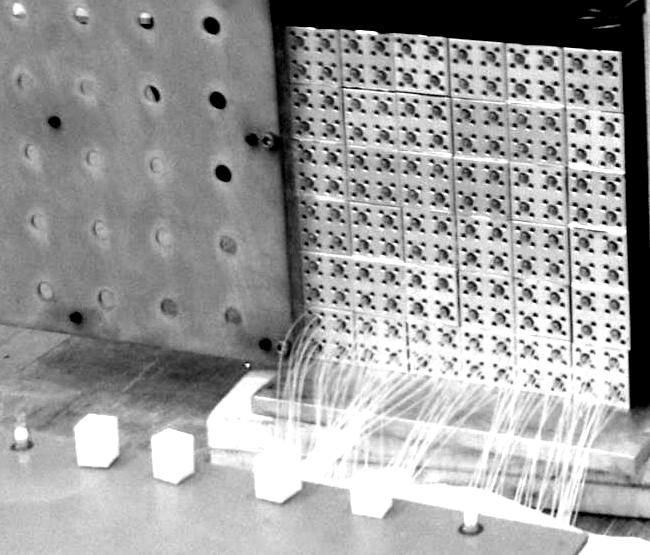
\includegraphics[width=0.5\linewidth]{images/illustrative/ecal-assembly-photo-opened.png}
    \caption{Фотография торцевой части ECAL NA64 со снятым кожухом}
    \label{fig:ecal-assembly-photo-opened}
\end{figure}

Все ячейки набраны из свинцовых пластин толщиной~$1.5~\text{мм}$
чередующихся с пластинами из полиметилметакрилата
толщиной $1.55~\text{мм}$ с бумажной проставкой $140~\text{мкм}$.
Предливневая часть состоит из 16-и слоёв, основная часть из 150-и.
Все пластины имеют перфорацию для пропускания светопроводящего волокна
(16 отверстий на ячейку) и армирующих стальных стержней (четыре отверстия).

Таким образом, калориметр имеет толщину соответствующую примерно 42
радиационным длинам ($\simeq42{,}4 X_0$) и мольеровский
радиус~$R_M\simeq1{,}8~\text{см}$, откуда следует, что при попадании
электрона в калориметр, его энергия
за счёт одного только тормозного излучения уменьшится в $e^{42}$ раз.
Практически, высокоэнергетический электрон инициирует
в веществе калориметра развитие электромагнитного ливня (каскада) за
счёт процессов образования пар, комптоновского рассеяния и
фотоэлектрического эффекта. 90\% энерговыделения сосредоточено
внутри цилиндрического объёма диаметром $36~\text{мм}$ -- в одной
ячейке в случае центрального падения.

Для задач калибровки калориметра важно, что \acrshort{mip} для
заряженных мюонов с энергией свыше нескольких десятков ГэВ
составляет $\simeq353~\text{МэВ}$ ($2{,}26~\text{МэВ}$ на слой).

%На рисунке приведена визуализация моделирования образования
%электромагнитного ливня в ECAL и профиль ливня \cite{grupenDetectors2008}
%Сигнал от предливневой части вводится в триггерную систему и служит в основном
%для отделения адронных событий.

Энергетическое разрешение калориметров определяется следующей
формулой, учитывающую вклад отдельных свойств детектора и считывающей системы:
% (символом "$\oplus$" обозначена прямая сумма)
\begin{equation}
    \frac{\sigma}{E} = \frac{a}{\sqrt{E}} \oplus b \oplus \frac{c}{E}.
    \label{eq:ecalResolution}
\end{equation}
В формулу включены феноменологические параметры $a, b, c$, отвечающие за
влияние эффектов различной природы \cite{CalorimetryPPhFabiola}:
\begin{itemize}
    \item $a$ -- стохастический член, отвечающий за фотостатистику,
    в который включены внутренние флуктуации в ливне, флуктуации
    в отдельных слоях и квантовые флуктуации сигнала,
    \item $b$ -- постоянный член отвечающий за флуктуации
    электроники (динодная система, зарядово-цифровые или
    амплитудно-цифровые преобразователи и т.д.),
    \item $c$ -- слагаемое отвечающее за ошибки калибровки,
    неоднородности сцинтиллятора и другие независящие от энергии
    факторы.
\end{itemize}

В общем, для гетерогенных калориметров типичное относительное
энергетическое разрешение лежит в
диапазоне~$5-20\%/\sqrt{E}$~\cite{CalorimetryPPhFabiola}.
При этом, основной вклад в
ухудшение разрешения вносят флуктуации в отдельном активном слое (число
заряженных частиц $n_{ch} \propto E/t$, где $t$ -- толщина слоя
поглотителя)~\cite{grupenDetectors2008, wigmansCalorimetry},
при этом стохастический член $a$ из $\eqref{eq:ecalResolution}$
изменяется как $\sigma_{samp}/E \propto \sqrt{t/E}$.
С целью её уменьшения стремятся увеличивать число слоёв,
уменьшая толщину отдельного слоя поглотителя.

В частности, чтобы получить представление о значениях энергетического
(а также координатного и углового) разрешения достижимых
практически в калориметре конструктивно-схожего типа, можно
обратиться к работам RD36. В техническом проекте~\cite{rd36-shashlik-1996}
приводятся оценки для калориметра свинец-полиметилметакрилат с
толщинами слоёв~$2~\text{мм}$ и $4~\text{мм}$ соответственно, и
стороной ячейки~$47~\text{мм}$. В этой работе отмечается сильная
зависимость энергетического разрешения ячейки калориметра от
координаты попадания первичной частицы
(рисунок~\ref{fig:shashlyk-correction-quote}, слева). С целью
компенсации эффекта,
вводится феноменологическая аппроксимация оценки энерговыделения
как функция координаты попадания первичной частицы, результаты которой
представлены на рисунке~\ref{fig:shashlyk-correction-quote}.

С учётом координатной коррекции, авторы указывают энергетическое
разрешение для случая, когда выход считывается
высокостабильным~\acrshort{pmt}
\begin{equation}
    \frac{\sigma}{E}(\%) = \frac{9.0 \pm 0.1}{\sqrt{E}} \oplus (1.0\pm0.3),
\end{equation}
т.е. для электрона~$100~\text{ГэВ}$ принципиальный предел энергетического
разрешения составляет~$\sigma =1.9~\text{ГэВ}$.

\begin{figure}
    \centering
    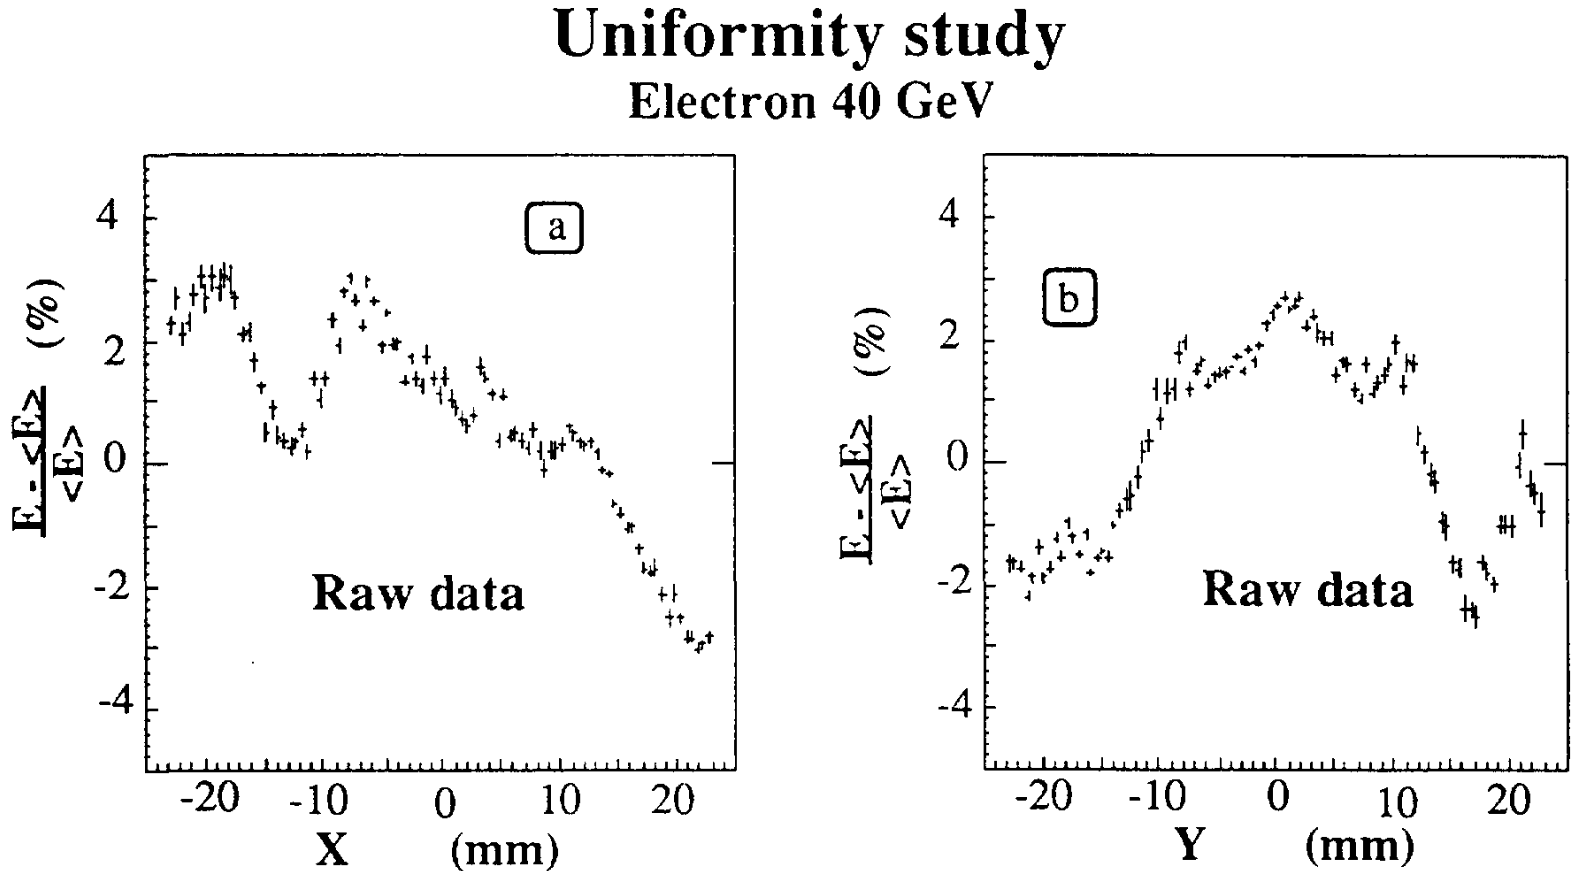
\includegraphics[width=0.48\linewidth]{images//illustrative/shashlyk-resolution-raw.png}
    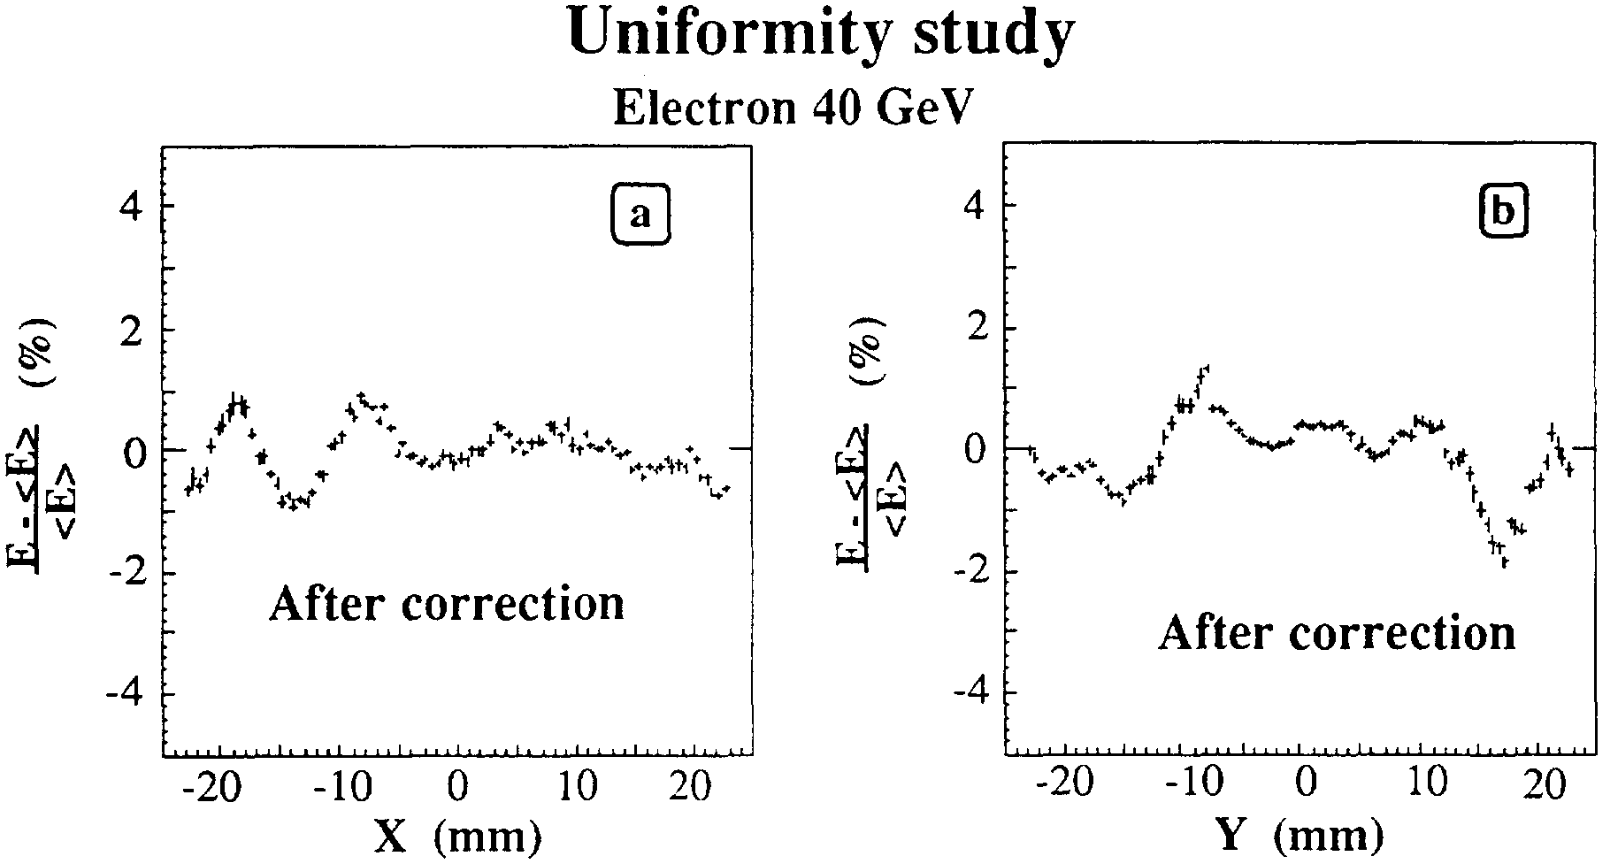
\includegraphics[width=0.48\linewidth]{images//illustrative/shashlyk-resolution-corrected.png}
    \caption{Зависимость оценки энерговыделения калориметра от координаты до и после коррекции согласно работе~\cite{rd36-shashlik-1996}}
    \label{fig:shashlyk-correction-quote}
\end{figure}

Результаты измерения энергетического разрешения
конструктивно-аналогичного калориметра опубликованы
в работе~\cite{chirkovzorin-compass-ecal}. За исключением
фотоприёмника и числа слоёв,
калориметр~COMPASS использует аналогичную NA64 конструкцию
ячеек, включая поперечные размеры, толщины слоёв, марку оптического
волокна и т.д. Полученная зависимость изображена на
рисунке~\ref{fig:chirkovzorin-compass-ecal}.
\begin{figure}
    \centering
    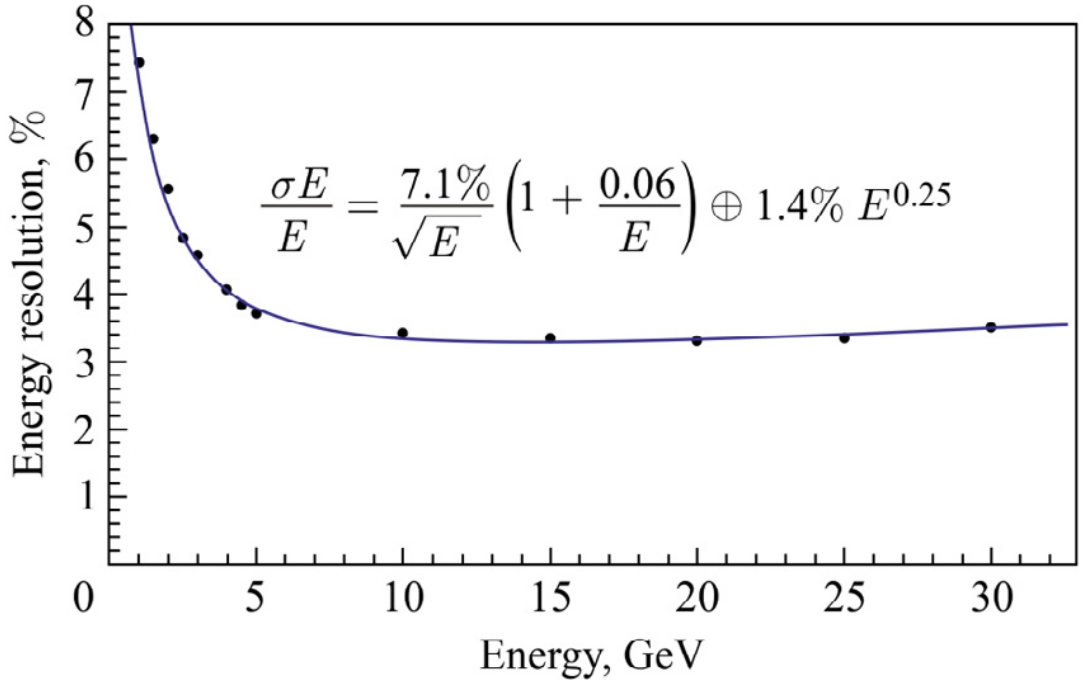
\includegraphics[width=0.5\linewidth]{images//illustrative/compassII-ecal.png}
    \caption{Относительное разрешение ECAL COMPASS фазы II, согласно~\cite{chirkovzorin-compass-ecal}}
    \label{fig:chirkovzorin-compass-ecal}
\end{figure}

Экстраполяция оценки относительного разрешения из этой работы до номинальной
энергии пучка NA64 ($100~\text{ГэВ}$) даёт значение $\simeq 5{,}14~\text{ГэВ}$.
Следует учесть, что практически разрешение должно быть несколько лучше,
поскольку линейный член в работе~\cite{chirkovzorin-compass-ecal}
отвечает за флуктуацию продольных утечек (и обуславливает ухудшение
относительного разрешения на рисунке~\ref{fig:chirkovzorin-compass-ecal}.

%---

%Для апостериорного вычисления коэффициентов
%выражения~\eqref{eq:ecalResolution}, прямая сумма $\oplus$ раскрывается
%следующим образом:
%\begin{equation}
%    \frac{\sigma (E)}{\langle E \rangle} = \sqrt{ \frac{c^2}{\langle E \rangle} + \frac{b^2}{\langle E \rangle^2} + \left( \frac{\sigma(p)}{p} \right)^2 },
%\end{equation}
%где $\sigma(p)/p$ --- импульсное разрешение установки.
% ^^^ проверить, взял https://arxiv.org/abs/hep-ex/0001020 , стр 11, ф-ла (42)

%Текущий раздел будет посвящён отысканию коэффициентов в
%формуле \eqref{eq:ecalResolution} и созданию параметрической модели
%электромагнитного ливня для дальнейших приложений.

\subsection{Адронный калориметр}

В качестве адронного калориметра в NA64 установлен
нескомпенсированный калориметр железо-полиметилметакрилат.
Калориметр имеет поперечную сегментацию $3\times3$
и состоит из четырёх независимых модулей. В рассматриваемых
в данной работе постановках эти модуле как правило ориентируются
вдоль по оси пучка и устанавливаются подряд, дополняя ECAL до
герметичной установки.

Конструктивно, каждый модуль калориметра выполнен в виде
сварной металлической конструкции, в которую помещаются
вкладыши со сборками сцинтилляционных пластин из ПММА обёрнутых
в металлизированный майлар, с выведенными наружу
сцинтилляционными волокнами, как показано на рисунке~\ref{fig:hcal-module}.

Толщина одной $192\times194~\text{мм}$ сцинтилляционной
пластины -- $4~\text{мм}$, поглотителя -- $25~\text{мм}$.
Во вкладыше пластины расположены с небольшим зазором для обеспечения
выхода волокна, так что общая длина одного модуля калориметра
состоящего из 48-и слоёв составляет $1500~\text{мм}$, обеспечивая,
таким образом длину ядерного взаимодействия $7.43 \lambda_I$.

% Плотности:
%   Сталь: 48*25 = 120 см
%   ПММА: 48*4 = 19.2 см
% Длины взаимодействия (PDG):
%   Сталь: \lambda_I = 132.1 г/см^3 => 16.77 см при плотности 7.874 г/см:3
%   ПММА:  = 83.0 г/см:2, плотность 1.16-1.20 г/см^3 => \lambda_I = 70 см
% Число ядерных длин = 120/16.77 + 19.2 / 70.3 = 7.43

\begin{figure}
    \centering
    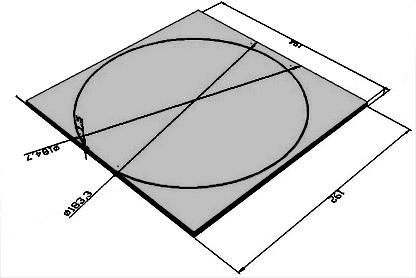
\includegraphics[width=0.3\linewidth]{images/hcal-cell-single-plastic-element.png}
    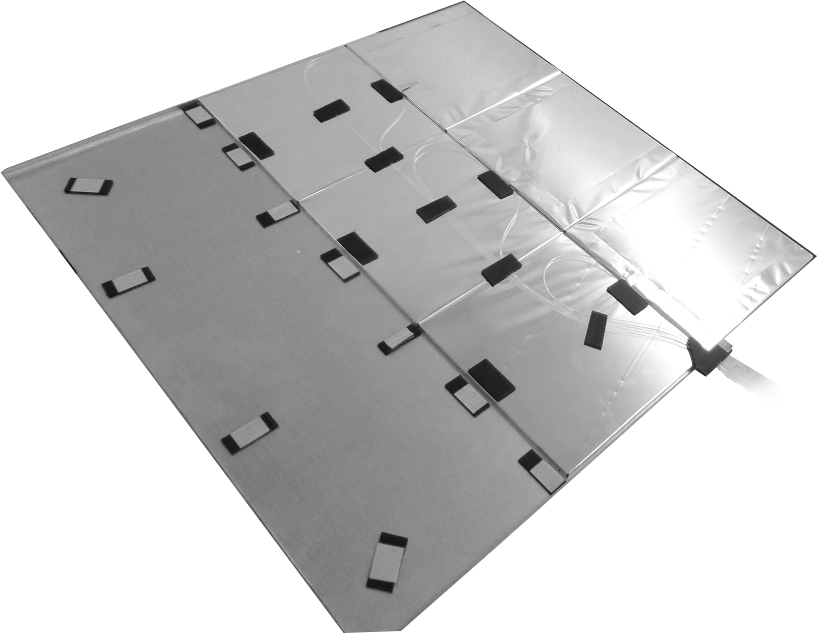
\includegraphics[width=0.3\linewidth]{images//illustrative/hcal-inlet-photo.png}
    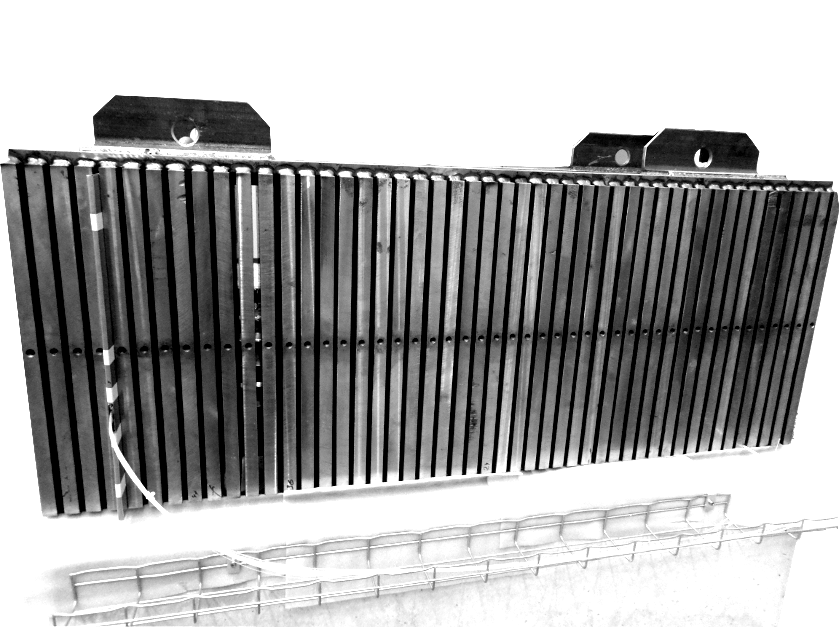
\includegraphics[width=0.3\linewidth]{images//illustrative/hcal-frame-photo.png}
    \caption{Схема укладки оптического волокна, фотографии вкладыша и сварного каркаса HCAL~\cite{PolyakovHCALDrawings-na64site}}
    \label{fig:hcal-module}
\end{figure}

Для задач калибровки калориметра важно, что \acrshort{mip} для
заряженных мюонов $\simeq1{,}55~\text{ГэВ}$ ($32{,}4~\text{МэВ}$ на слой)

Волокна от пластин отвечающих выделенному продольному направлению
соединяются на фотокатоде одного~\acrshort{pmt}, предоставляя
информацию об одной <<ячейке>>.

Детектор играет важную роль в случаях, когда в электромагнитном
калориметре происходит происходит адронизация компонент
ливня (<<адронный хвост>>) -- в
основном это реакции с выходом пионов: фотоядерные
реакции~$\gamma + Z \rightarrow \pi + Z$ (десятки мб на ядро Pb),
фотодезинтеграция ядер, фоторождение $\eta$-мезонов ($0{,}01$ мб),
адронизация через $\rho$-мезон и т.д. Для статистики
свыше~$10^{12}$ играет роль также нейтральная компонента
пучка ($\pi^0$, $K^0$, пробивные $\gamma$-кванты), которые также
можно идентифицировать в HCAL опираясь на пространственные
характеристики ливня.

\subsection{Микроструктурные детекторы}

В качестве трековых детекторов высокого разрешения в NA64 применяются
детекторы GEM (Gas Electron Multiplier)~\cite{gems-sauli} и 
MicroMega (MICRO-MEsh GAseous Structure)~\cite{na64-BANERJEE201872}. Оба типа детекторов
относятся к семейству т.н. \emph{микроструктурных детекторов с газовым
усилением}. Общая идея регистрации заряженной частицы этими детекторами
состоит в регистрации электронной ионизационной лавины развивающийся
в газовой смеси при прохождении заряженной частицы планарной структурой
из тонких (десятки-сотни мкм) электродов.

Основное отличие GEM и MicroMega заключается в конструктивной реализации
принципа газового усиления. В детекторах GEM усиление реализуется за счёт
локального увеличения напряжённости вблизи отверстий перфорирующих тонкую
полимерную фольгу с металлизацией, на которую подаётся разность потенциалов.
Считывание затем производится с металлизированного катодного слоя на
стенке газового объёма, как изображено на рисунке~\ref{fig:gem-charge-collection}.
\begin{figure}
    \centering
    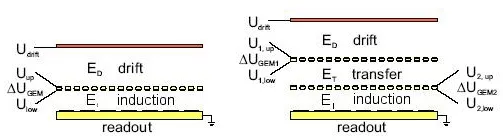
\includegraphics[width=0.65\linewidth]{images//illustrative/gem-charge-collection.png}
    \caption{Схематическое изображение гальванического усиления и зарядового
    считывание в объёме детектора GEM \cite{gems-compass}}
    \label{fig:gem-charge-collection}
\end{figure}
В детекторах MicroMegas, напротив, усиление происходит в узком газовом
зазоре между анодной платой и тонкой металлической сеткой, создающей
градиент электрического поля как показано на рисунке~\ref{fig:mumega-charge-collection}.
Таким образом, в GEM принцип газового
усиления реализуется каскадом электродов, а MicroMegas --
однородной областью лавинного умножения непосредственно над анодом.
\begin{figure}
    \centering
    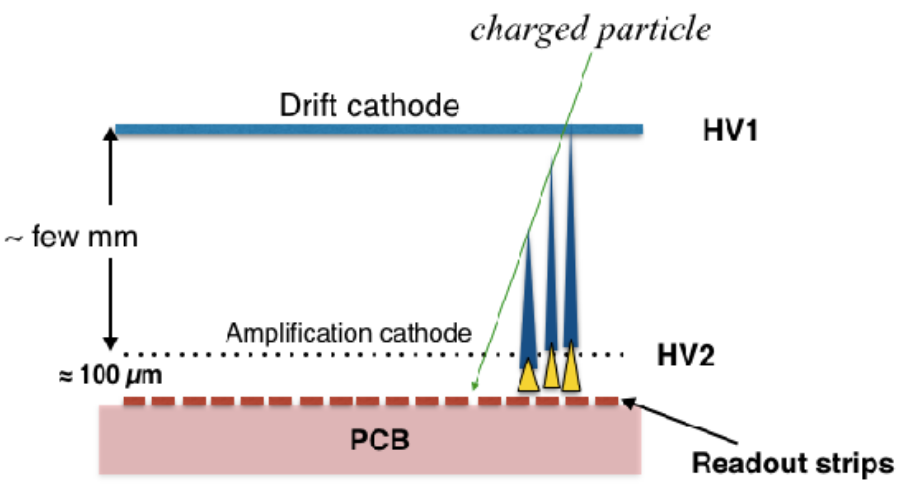
\includegraphics[width=0.65\linewidth]{images//illustrative/mm-charge-collection-example.png}
    \caption{Регистрация треков в рабочем объёме детектора MicroMega \cite{na64-BANERJEE201872}}
    \label{fig:mumega-charge-collection}
\end{figure}

В NA64 оба типа детекторов представлены в микростриповом исполнении --
анод выполнен в виде полос нанесённых литографическим методом на тонкую
подложку (каптон). Такая плоскость даёт информацию
о координате вдоль одного направления. Для восстановления пространственной
точки попадания частицы в рабочий объём плоскости монтируются в виде
отдельных станций состоящих из двух плоскостей, дающих проекционную
информацию о месте развития электронной лавины вдоль пары перпендикулярных
координатных осей (годоскопический принцип).

%TODO: размеры
Рабочий объём детекторов продувается смесью $\text{Ar}/\text{CO}_2$ 80/20\%
при атмосферном давлении.

Считывание электрических сигналов осуществляется посредством
демультиплексирования амплитудных импульсов со всего массива полос на
плоскости и последующего преобразования амплитудного сигнала в цифровую форму.
За аналоговое демультиплексирование отвечает интегральная
микросхема APV~\cite{apv-jones},
в то время как сэмплирующее амплитудно-цифровое преобразование осуществляется
микросхемой MSADC.

Не смотря на хорошее координатное разрешение ($\simeq 200-250\text{мкм}$) и
устойчивость отклика при высоких загрузках, микроструктурные
детекторы NA64 имеют ограниченную площадь чувствительной поверхности и
применяются в основном в системе мечения.

\subsection{Детекторы на основе тонкостенных трубок}

С целью увеличения аксептанса трекер NA64 оснащён станциями состоящими из
тонкостенных дрейфовых трубок~(\emph{straw})~\cite{straws-volkov2019, straws-peshekhonov2015}.
Каждая трубка представляет собой цилиндрическую поверхность выполненную
из гибкой полимерной плёнки с металлизацией (катода) с протянутой
вдоль её оси проволокой-анодом. Через массив трубок продувается
смесь $\text{Ar}/\text{CO}_2$ (80/20\%) при атмосферном давлении.

Принцип измерения координат основывается на регистрации времени дрейфа
ионизационных электронов к аноду отдельной трубки, как показано
на рисунке~\ref{fig:straws-measurement}.

\begin{figure}
    \centering
    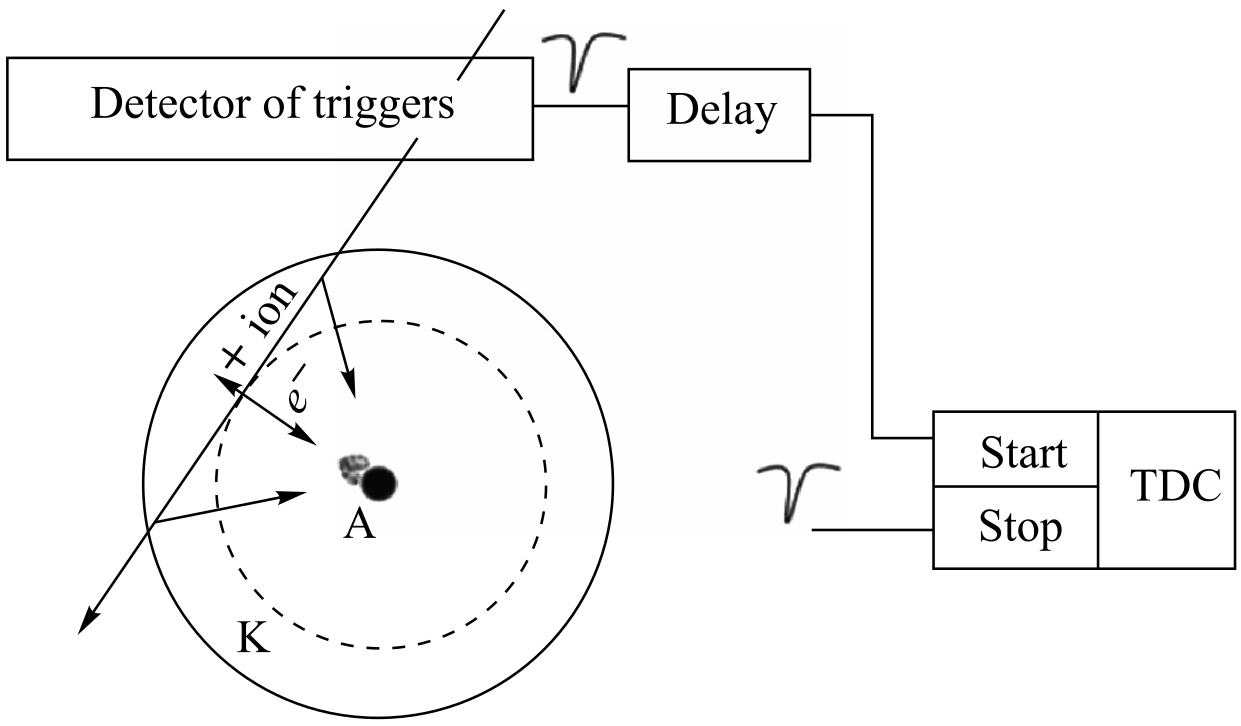
\includegraphics[width=0.5\linewidth]{images//illustrative/strawa-principle.png}
    \caption{Схема измерения времени дрейфа ионизационных электронов~\cite{straws-peshekhonov2015}}
    \label{fig:straws-measurement}
\end{figure}

Для NA64 были изготовлены станции трёх типов:
\begin{itemize}
    \item $200\times200~\text{мм}$ С внутренним диаметром
    трубок $6{,}02 \pm 0{,}025~\text{мм}$, и толщиной
    стенки~$62~\text{мкм}$, с металлизацией алюминием толщиной $500~\mathring{\text{A}}$.
    В качестве анода используется позолоченная вольфрамовая проволока диаметром $30~\text{мкм}$.
    \item $200\times200~\text{мм}$ С внутренним диаметром
    трубок $2 \pm 0{,}025~\text{мм}$, и толщиной
    стенки~$67~\text{мкм}$, с металлизацией алюминием толщиной $200~\text{нм}$
    и дополнительным покрытием защитным слоем графитополиуретана толщиной~$6~\text{мкм}$.
    В качестве анода используется позолоченная вольфрамовая проволока диаметром
    $20~\text{мкм}$.
\end{itemize}

С точки зрения трекинга, измеренное время сигнала $t$ с анода задаёт
изохронную цилиндрическую поверхность с радиусом $r = t v$, где
$v$ -- характерная скорость дрейфа электронов в газовой смеси.
Алгоритмически, такие изохронные поверхности способны приводить к
неоднозначностям при реконструкции трека, поэтому станции обычно состоят
из массивов тонкостенных дрейфовых трубок или являются частью
многоступенчатого трекера.

\subsection{Номенклатура детекторов}

С целью охвата всей номенклатуры детекторов в рамках программных
моделей имеющих дело с данными эксперимента в общем (и с моделью
события в частности), необходимо учесть следующие обстоятельства,
связанные с представлением данных на низком уровне 

На уровне отдельных измерений, состав (тип и топология)
данных \emph{полностью} определяется основной микросхемой (\emph{чипом})
обслуживающей карты осуществляющей преобразование сигналов.
Это означает, в частности, что сигналы оцифрованные с калориметра,
пучкового счётчика, вето-детектора и мюонного счётчика будут
содержать одну и ту же информацию в смысле типа данных. В то же
время, сигнал от микроструктурных детекторов -- будь
то GEM или MicroMega будут иметь другой тип данных.

Таким образом, с точки зрения физического представления данных,
целесообразным является помещение показаний от одного типа в
коллекцию. Тогда статический аллокатор коллекции будет иметь дело
с данными одного типа, что уменьшит фрагментацию данных и
улучшит локальность кэширования. Дополнительным преимуществом
такого решения является возможность итерировать всю такую коллекцию
в рамках одной лексемы -- во многих случаях прикладные алгоритмы
(обработчики конвейера данных) нуждаются в доступе такого вида.
Например, алгоритм вычисления сигнала нулевого уровня
совершенно агностичен к тому, к какой станции,
или к какому типу детекторов относится набор сэмплов.

Следующим важным делением детекторов является деление
по \emph{семейству} (англ. \emph{kin}). В системе сбора данных NA64
приняты обозначения, некоторые из которых приведены в
таблице \ref{tab:detector-names-examples}.

\begin{table}[ht]
\centering
\begin{tabular}{r|cl}
Наименование & Чип     & Описание \\ \hline
          S1 & MSADC   & Первый пучковый счётчик \\
        VETO & MSADC   & Вето-детектор \\
        ECAL & MSADC   & Электромагнитный калориметр \\
        GM03 & APV     & Газовый электронный умножитель №3 \\
        MM02 & APV     & Микросеточный газовый детектор №2  \\
        ST06 & NA64TDC & Трубчатый дрейфовый детектор №6
\end{tabular}
\caption{Примеры наименований детекторов}
\label{tab:detector-names-examples}
\end{table}

Наконец, необходимо индексировать отдельные чувствительные
элементы детектора. В зависимости от семейства к которому принадлежит
детектор, это могут быть ячейки калориметра, проекционные
плоскости трековых детекторов, трубки газовых детекторов.

В результате, дескриптор уникально идентифицирующий чувствительный
элемент детектора должен содержать следующую семантику (в порядке
убывания общности):

\begin{enumerate}
    \item Идентификатор типа микросхемы (чипа, <<chip>>), определяющий
    тип данных,
    \item Идентификатор семейства детектора (<<kin>>), дающий информацию о
    физическом смысле сигнала,
    \item Номер станции, для уникальной идентификации детектора в
    пределах одного семейства,
    \item Нагрузку (<<payload>>), содержащую информацию о конкретном
    чувствительном элементе детектора, в зависимости от чипа или семейства.
\end{enumerate}

Для калориметров и сегментированных детекторов с \acrshort{pmt},
нагрузке достаточно содержать три индекса, идентифицируюших
ячейку или сегмент детектора.

Для микроструктурных трековых детекторов нагрузка должна содержать
информацию об ориентации проекционной плоскости детектора и номер
чувствительного элемента.

Простой расчёт показывает, что всю номенклатуру детекторов NA64
можно уместить в множестве мощностью не более $2^{64}$ значений,
что позволяет, в принципе, использовать номерной идентификатор
для кодирования дескриптора детектора. Это позволяет свести
операции запроса и поиска элементов коллекций до простых
операций с целым числом фиксированной длины, осуществлять выборку
элементов применением быстрых побитовых операций и т.д.


\begin{comment}
\subsection{Моделирование э/м ливня}

Для оценки вклада в разрешения факторов обусловленных физикой ливня
воспользуемся эмпирической формулой разрешения для слоистого калориметра с
заданной геометрией~\cite{delPeso1989-sampling-calorimeters}:
\begin{equation}
    \frac{\sigma_{sampl}}{E}(\%) = \frac{3.5}{\sqrt{E}}
        \cdot \left( \frac{t}{X_t} \right)^{\alpha}
        \cdot \left( \frac{s}{X_s} \right)^{\beta},
\end{equation}
где $t, X_t, s X_s$ --- толщина и радиационная длина слоёв сцинтиллятора и
свинца, соответственно, а $\alpha, \beta$ --- некоторые подстроечные  % e.g. alpha=0.67, beta=-0.3
коэффициенты, которые обычно определяются из МК-модели
калориметра (в оригинальной работе~\cite{delPeso1989-sampling-calorimeters}
моделирование производилось в пакете EGS4, 1988). % TODO использующего модели
Современный (напр. 4.10.6) Geant4 предоставляет возможность использовать
различные комбинации моделей процессов электромагнитного ливня с тем чтобы
обеспечить наилучшее согласие в известном диапазоне энергий.

Для моделирования развития ливня зададим геометрию калориметра в виде цилиндра
составленного из круговых пластин сцинтиллятора и свинца с толщинами
соответствующих слоёв ECAL. Получившуюся модель цилиндрического калориметра
сегментируем по $\rho, \phi, z$ с тем чтобы для заданной энергии инициирующей
частицы получить \emph{энергетический профиль} э/м ливня в виде функции со
следующей факторизацией:

\begin{equation}
    \dd E(\rho, z) = E/2\pi \cdot f(\rho) \dd \rho \cdot f(z) \dd z.
    \label{eq:emshowerFac}
\end{equation}

Нужно заметить, что факторизация \eqref{eq:emshowerFac} справедлива только для
перпендикулярного направления движения частицы по отношению к пластинам
калориметра. В силу анизотропии размещения поглотителя в веществе калориметра,
такая факторизация перестаёт работать.
% ^^^ интересным приложением может быть реконструкция угла падения частицы на
% основе такой информации --- хотя вклад от \phi по-видимому нельзя
% факторизовать, вероятно возможно подобрать декомпозицию другого рода...

\subsection{Продольный профиль э/м ливня}

Известно, что продольный профиль ливня хорошо описывается
$\Gamma$-распределением \cite{Longo1975EMCSim}:

\begin{equation}
    \left\langle \frac{1}{E} \frac{\dd E(z)}{\dd z} \right\rangle = f(z) = \frac{(\beta z)^{\alpha-1} \beta \exp(-\beta t)}{\Gamma (\alpha)},
\end{equation}
где $\alpha$ регулирует форму продольного профиля а $\beta$ --- масштаб.  %< TODO: "масштаб"?
Центр масс $\langle z \rangle$ энергетического распределения связан с этими
параметрами как $\langle z \rangle = \alpha / \beta$, а максимум может быть
выражен как $\max f(z) = (\alpha - 1)/\beta$.
\end{comment}